
\section{Descripción}

Las formaciones ferroviarias cuentan con varios Sistemas Instrumentados de Seguridad (SIS) a bordo con el objetivo de supervisar el correcto funcionamiento de los subsistemas críticos como por ejemplo, la protección de coche a la deriva, el sistema de hombre vivo o la seguridad de puertas. \\

Estos sistemas están diseñados para que, ante la detección de una falla crítica, se produzca la detención de la formación de manera inmediata. Esto se logra controlando las señales de Corte de Tracción (CT) y de Freno de Emergencia (FE). En esta situación, la formación puede ser remolcada o bien, desactivar todos los SIS bajo estricta supervisión y continuar andando con el control manual del conductor hasta una estación cercana para descender a los pasajeros y luego a un taller para ser reparada. \\

El Sistema de Aislamiento Limitado/Total, por sus siglas SAL/T, es un equipo que permite una circulación controlada y más segura de la formación cuando uno de los SIS se encuentra en falla. Al  activar el Modo Aislado Limitado (MAL), el SAL/T va a deshabilitar solamente el SIS que está en fallo y controlar las señales de CT y FE para poder continuar con la circulación de la formación. Para hacerlo de manera segura, el SAL/T va a contar con múltiples fuentes de medición de la velocidad de la formación y va a activar las señales de CT y FE para frenarla en caso de que se excedan los límites estipulados. En el Modo Aislado Total (MAT), se libera la velocidad de precaución y puede ser solamente aplicado por personal superior en el caso que la formación se encuentre sin pasajeros y muy alejada del centro reparador. Ambas activaciones deben ser registradas dentro del equipo así como también cualquier falla detectada, cambio de configuración en las velocidades permitidas o cualquier evento significativo para la seguridad de la formación.\\

Además, el SAL/T cuenta con otras funcionalidad como la comunicación con el conductor a través de una interfaz donde se muestra el estado de los SIS, la velocidad medida en todo momento y un indicador de la zona donde se encuentra la formación. En caso de no contar con una medición de velocidad válida y activar el MAL, el SAL/T entra en Modo Intermitente (MI) y controla la formación activando y desactivando la tracción y el freno acorde a los perfiles de tiempos preconfigurados según las características de la formación para no exceder ciertas velocidades de precaución. Desde el panel formal, el conductor puede seleccionar distintos perfiles intermitentes.  También, el SAL/T tiene la posibilidad de conectarse con una central operativa para informar su estado y recibir remotamente instrucciones. \\

Este equipo es considerado un sistema crítico ya que, en caso de fallar, puede conllevar pérdidas de vidas humanas o daños importantes tanto de propiedades como del entorno. \\

En el 2019, el Ingeniero Iván Di Vito presentó un prototipo de este sistema con pruebas de campo en los talleres de Trenes Argentinos siguiendo las fases y recomendaciones de la norma UNE-EN 50126 \cite{norma_50126};  ``Aplicaciones ferroviarias. Especificación y demostración de la fiabilidad, la disponibilidad, la mantenibilidad y la seguridad (RAMS)''. En el año 2022, los ingenieros Fernando Iglesias y Matías Sambrizzi realizaron el trabajo “Central Operativa para el SAL/T” donde se desarrolló la central operativa para monitorear, controlar y configurar múltiples formaciones equipadas con el SAL/T de manera remota desde un centro de operaciones. Ambos trabajos fueron desarrollados con el acompañamiento del Grupo de Investigación en Calidad y Seguridad de las Aplicaciones Ferroviarias (GICSAFe) como trabajo final de grado de Ingeniería Electrónica en la Universidad de Buenos Aires teniendo como directores al Dr. Ing. Ariel Lutenberg y al Dr. Ing. Pablo Gomez. \\

En este trabajo, se busca hacer un rediseño del prototipo del SAL/T implementando algunas mejoras sugeridas por Trenes Argentinos en el pliego de especificaciones técnicas ET.SO.No 046/18–E3 del 2022, utilizando un microcontrolador y componentes más modernos y un firmware basado en un sistema operativo de tiempo real que resulte más portable que el actual. A continuación se muestra un diagrama en bloques del sistema a desarrollar: 


\begin{figure}[H]
    \centering
    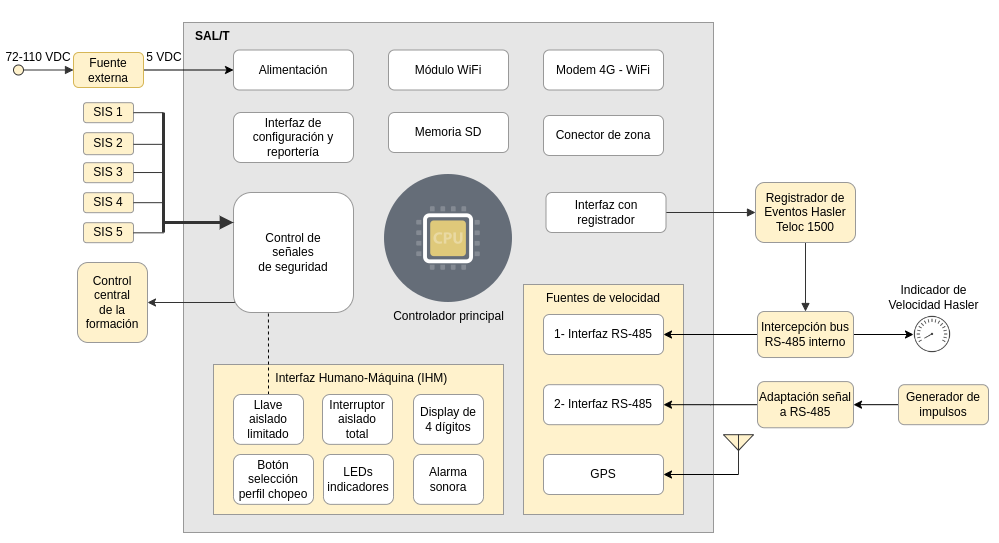
\includegraphics[width=\linewidth]{img/diagrama_bloques.png}
    \caption{Diagrama en bloques del SAL/T}
    \label{fig:block_diagram}
\end{figure}

También se muestra la interfaz humano-máquina (IHM) diseñada para comunicarse con el conductor de la formación:

\begin{figure}[H]
    \centering
    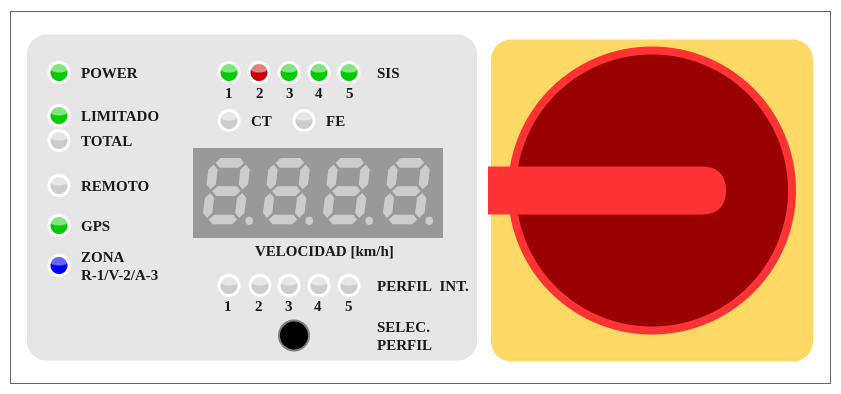
\includegraphics[width=\linewidth]{img/panel_frontal.png}
    \caption{Interfaz humano-máquina del SAL/T}
    \label{fig:him}
\end{figure}